%************************************************
\chapter{Problems to Solve}\label{ch:problems_to_solve}
%************************************************

\section{Build a Reflective Knowledge Substrate}

The assumption that we introduced in
Section~\ref{sec:introducing_reflection_early_in_the_process},
``Introducing Reflection Early in the Process'', requires that changes
in our knowledge representation can be traced and compiled into other
representations, such as the reflective event representations used in
learning to accomplish goals.

\subsection{General Parallelism and Concurrency}

\begin{figure}[bth]
  \center
  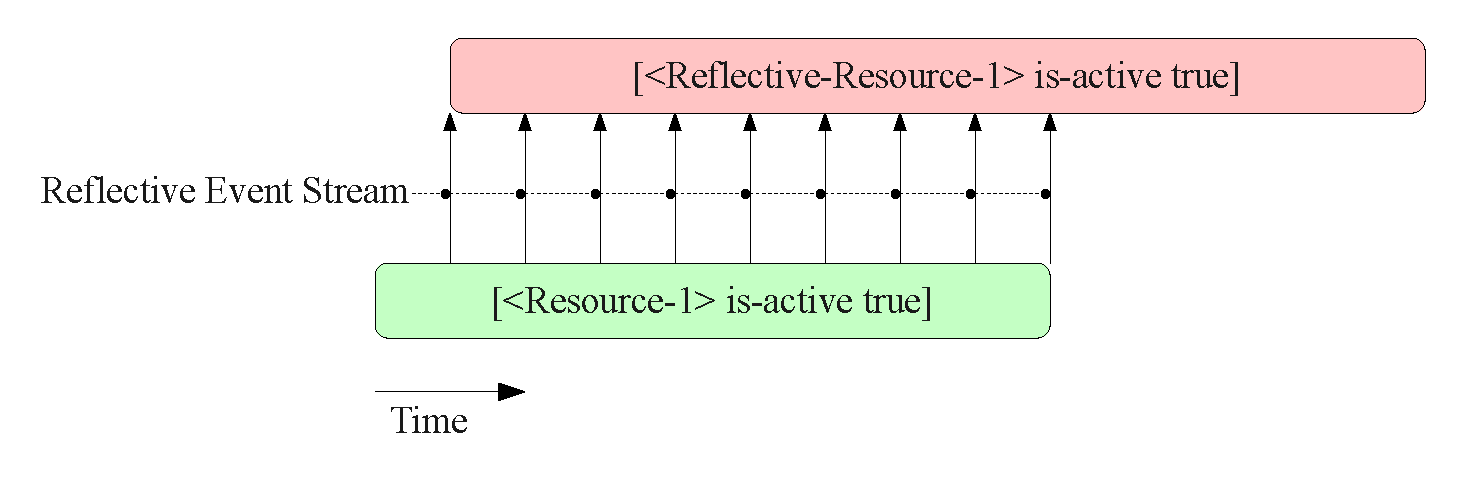
\includegraphics[height=3cm]{gfx/concurrent_parallel_reflection_efficiency}
  \caption[Concurrent parallel reflection efficiency]{Concurrent parallel reflection efficiency.}
  \label{fig:concurrent_parallel_reflection_efficiency}
\end{figure}

See Figure~\ref{fig:concurrent_parallel_reflection_efficiency}.



\subsection{Automatic Collection of Audit Trails for All Processes}

\subsection{Program as Data}

The ability for a process to manipulate a program as data makes it
easier for that process or a user to read, edit, and write programs as
they are debugged.


\section{Layered Reflective Problem Solving}

\subsection{Analogy between Physical Goals and Planning Goals}


\section{Learning by Credit Assignment}

\subsection{Use Reflective Representations for Better Models of Learning}

\subsection{Tracing Knowledge Provenance for Credit Assignment of Success or Failure}



